\documentclass[12pt,letterpaper]{article}

\usepackage[bookmarks=true]{hyperref}
\usepackage{graphicx}
\usepackage{geometry}
\usepackage{fontspec}
\usepackage{xunicode}
\usepackage{xltxtra}
\usepackage{color,colortbl}
\usepackage{url}
\usepackage[table]{xcolor}
\usepackage{multirow}
\usepackage{xtab}
\usepackage[final]{pdfpages}
\usepackage{subfigure}
\usepackage{amsmath,amssymb}


\definecolor{Gray}{gray}{0.9}

\defaultfontfeatures{Mapping=tex-text} % converts LaTeX specials (``quotes'' --- dashes etc.) to unicode

\setromanfont [Ligatures={Common}]{Cardo}
\setmonofont{Inconsolata}

% Set your name here
\def\name{Patrick J. Martin}

% Replace this with a link to your CV if you like, or set it empty
% (as in \def\footerlink{}) to remove the link in the footer:
\def\footerlink{}

% The following metadata will show up in the PDF properties
\definecolor{darkblue}{rgb}{0.0,0.0,0.5}
\hypersetup{
  colorlinks = true,
  linkcolor=darkblue,
  urlcolor = darkblue,
  pdfauthor = {\name},
  pdftitle = {\name: PJM Application},
  pdfpagemode = UseNone
}

\geometry{
  body={6.5in, 8.5in},
  left=1.0in,
  top=1.0in,
  bottom=1.0in
}

\subfigcapmargin = .5cm

% Customize page headers
\pagestyle{myheadings}
\markright{\name}
\thispagestyle{empty}

% Custom section fonts
\usepackage{sectsty}
\sectionfont{\rmfamily\mdseries\Large}
\subsectionfont{\rmfamily\mdseries\large}

% Don't indent paragraphs.
\setlength\parindent{0em}

% Make lists without bullets
\renewenvironment{itemize}{
  \begin{list}{}{
    \setlength{\leftmargin}{1.5em}
  }
}{
  \end{list}
}

% courtesy D. Hovemeyer
\newenvironment{denseItemize}{%
\begin{list}{}{\setlength{\itemsep}{0.4em}\setlength{\leftmargin}{1.5em}\setlength{\parsep}{0in}}}{\end{list}}
%\setlength{\topsep}{.1mm}

\begin{document}

\pagestyle{myheadings}
\markright{\name---Project 4: Training a Smart Cab to Drive}
\thispagestyle{empty}

%{\LARGE \name} \\
%\smallskip
%\smallskip
{\Large Project 4: Training a Smart Cab to Drive} \\ 
Patrick Martin \\
\rule{\columnwidth}{1pt}

\vspace{1em}

In this project, I applied reinforcement learning techniques to design and simulate a smart cab agent operating.

\subsection*{Testing and Design Tasks}

To ensure that my development environment was complete, I implemented an agent that randomly selects an action without any ``smarts.'' 
This agent uses a discrete uniform distribution over the four possible actions: \verb|None|, \verb|left|, \verb|right|, and \verb|forward|.
It is clear from this strategy that the agent will bounce around the board due to the randomness of its action selection and the randomness of the environment (traffic lights and other agents).
The agent usually arrives at the final goal; however, there is no guarantee on timing performance. 
I let the agent run five times and tabulated the simulation deadline and the number of steps to completion:

\begin{figure}[h!]
\begin{center}
    \begin{tabular}{| c | c |}
    \hline
    \textbf{Deadline} & \textbf{Steps to Completion} \\ \hline
    20 & 168 \\ \hline
    40 & 120 \\ \hline
    25 & 7 \\ \hline
    30 & 22 \\ \hline
    40 & 118 \\
    \hline
    \end{tabular}
\end{center}
\caption{Tabulated data from several runs where the smart cab agent uses a full random action selection.}
\label{fig:randomtable}
\end{figure}

As Figure \ref{fig:randomtable} illustrates, two out of the five runs completed before the deadline, but it is likely due to the right combinations of initial conditions.
An open-loop algorithm will clearly not work for this task. \\

The driving agent state should be composed of environment variables that facilitate proper decision making.
The chosen state must balance the information required to solve the problem with the space complexity of the Q-learning algorithm.
Some input data may not be needed, which will create a more efficient learning algorithm. \\

I studied the available agent data and experimented with my implementation of the Q-learning algorithm.
At a minimum the state should include the intersection light, $\{\verb|green|,\verb|red|\}$, the direction of the next waypoint, $\{\verb|forward|,\verb|left|,\verb|right|\}$.
I added a new implicit state, the intersection traffic, based on the status of each path available to the agent.
A full state space would have used all three options for each direction; however, I chose to abstract them as a binary value: $\verb|true| := $ there is a vehicle on that path, $\verb|false|:=$ the path is clear.
Although I lose some information, the state space would have expanded to 384 states, which would take longer to explore.
I created the state space by building a Cartesian product in my Python code, \verb|itertools.product()|, resulting in 48 states.

\subsection*{Q-Learning Design and Implementation}

The cornerstone of the Q-learning algorithm is the construction of a {\bf Q-table}, which stores the value of each state-action pair.
This table starts with all entries at $0.0$.
Every time the smart cab agent takes an action from a state, it earns a reward from the environment, $R$.
Q-learning uses this reward and the current Q-table values to compute new values for the next iteration.
More formally: given current and next states, $s,s'\in S$, an action $a\in \mathcal{A}=\{\verb|None|,\verb|left|,\verb|right|,\verb|forward|\}$, at time step $k$ the estimate of the Q-value, $\tilde{Q}$ is computed by:
$$
	\tilde{Q}_{k+1}(s,a) = (1-\alpha_k)\tilde{Q}_{k}(s,a) + \alpha_k[R_k + \gamma \max_{a'\in\mathcal{A}}\tilde{Q}_k(s',a')].
$$
This particular form of the algorithm assumes that I am using the adjustable learning rate, $\alpha_k$, given by:
$$
	\alpha_{k+1} = \frac{1}{\alpha_k}, \textrm{ with } \alpha_0 = 1.
$$
Adopting this learning rate adjustment equation was in class as a strategy to make approximate Q-values converge to their expected value. \\

The implementation of my Q-table is a dictionary data structure that maps state-action tuples to their Q-value entry. For example, one of my chosen entries in the Q-table would look like:
\begin{center}
	\texttt{(('green', False, False, False, 'forward'), 'forward')}
\end{center}
that represents an intersection with a green light, no traffic, a waypoint goal that is in front of the cab and the agent takes the \verb|forward| action. \\

An agent running the Q-Learning algorithm stops taking random actions and takes smarter actions based on its prior performance.
The data in Figure \ref{fig:randomtable}, demonstrated that the random selection policy had no reasonable guarantee on reaching the destination in the desired time.

\subsection*{Q-Learning Algorithm Tuning}

Since my chosen state space has 48 states, I used the $\epsilon$-greedy exploration selection strategy to explore as much of the state as possible using a changing exploration probability, $\epsilon$.
In the lectures, I learned that using this technique (with inifinite exploration) guarantees that $\tilde{Q}\rightarrow Q$ and the approximate policy, $\tilde{\pi}$, approaches the optimal policy, $\pi^*$.
The $\epsilon$-greedy exploration action selection algorithm takes the following form:
$$
	\tilde{\pi}(s) = \left\{\begin{array}{c} \arg \max_a \tilde{Q}(s,a), \ 1-\epsilon \\ rand(\mathcal{A}), \ \epsilon \end{array}\right.
$$
where $rand(\mathcal{A})$ represents the random action selection used at the beginning.
In reinforcement learning, there is always a trade off between exploration and exploitation of knowledge.
If you do not explore, then you have limited knowledge; however, if all you do is explore, then you will not gather consistent enough knowledge for learning the optimal policy. \\

My particular $\epsilon$-greedy algorithm adjusts the value of $\epsilon$ as each trial runs according to:
$$
	\epsilon_{k+1} = \frac{1}{\sqrt{k}}, \ k=1,2,\cdots,n_{d},
$$
where $n_{d}$ is the deadline of a trial, i.e. 30, 40, etc.
The only value that is fixed for a simulation run is the discount factor, $\gamma$.
I used this parameter to tune the learning of the agent over several runs.
Figure \ref{fig:gammaplot} plots the success rate of my learning agent (using 100 trials per run) over the discount factor.
It is clear from the plot that lower $\gamma$ values result in better average success rates.

\begin{figure}[h!]
	\centering
	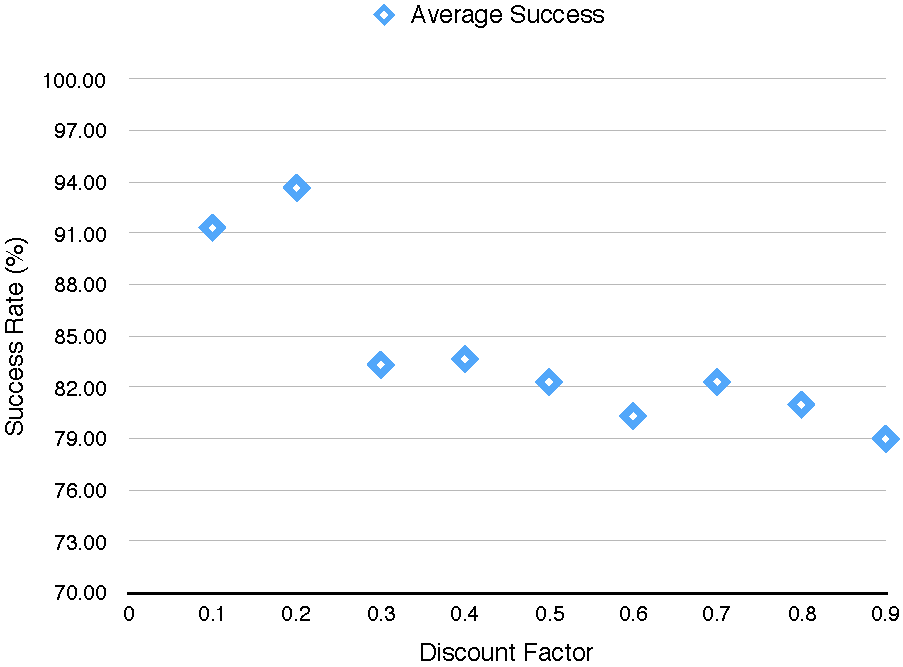
\includegraphics[width=0.75\textwidth]{SmartCabData.pdf}
	\caption{This plot shows how the success rate for my learning algorithm depended on $\gamma$. Each data point is the average success rate for 3 simulations runs, where each run had 100 trials.}
	\label{fig:gammaplot}
\end{figure}

Using this data, I chose my final discount factor to be $\gamma=0.2$.
This value, in combination with my $\epsilon$-greedy strategy with ``fading'' $\alpha$, resulted in a smart cab that consistently performs above 90\% for getting to the destination before the deadline.

\end{document}